\chapter{宠物养成机制：转生、融合与蛋喂养}

如果说上一章回答的是“宠物怎样长”，那么本章回答的是“宠物怎样被改造”。在当前系统中，转生、融合和蛋喂药并不是彼此独立的补丁，而是一条连续的养成流水线：原宠可以先通过转生改变成长档结构，也可以通过融合生成蛋基础成长，再经喂药与孵化映射为新的成长档，最终重新进入普通成长过程。因此，本章的重点不只是逐个介绍规则，而是把这些规则写成可组合的离散模型。

\section{转生模型}

\subsection{转生输入与总体结构}

转生模块的输入包括原宠成长率 $\bm{g}=(g_1,g_2,g_3,g_4)$、MM 向量 $\bm{m}=(m_1,m_2,m_3,m_4)$、宠物等级 $L_v$、转生次数以及转生能力上限。当前工具中，首转默认上限为 $150$，二转默认上限为 $200$，但这一上限允许人工覆盖，因此在论文中将其统一记为参数 $A_{\max}$。

转生并不是直接给出高等级宠物的最终面板，而是先生成一组新的基础成长率，再让该成长率像普通宠物一样经历后续出生与升级流程。若将转生后的确定性成长率记作 $\bm{g}^{(new)}$，则转生的逻辑链为
\begin{equation}
    (\bm{g},\bm{m},L_v,\text{转生次数},A_{\max})
    \longrightarrow A
    \longrightarrow \bm{g}^{(new)}
    \longrightarrow \text{普通成长流程}.
\end{equation}
其中 $A$ 即当前实现中的转生能力值，对应项目内部变量 \code{ans}。

\subsection{Rank、Fx 与转生能力值}

设原宠总和为
\begin{equation}
    T_2 = \sum_{i=1}^4 g_i,
\end{equation}
MM 总和经上限裁切后为
\begin{equation}
    T_1 = \min\left\{\sum_{i=1}^4 m_i,\,150\right\}.
\end{equation}
首转时，原宠 Rank 按普通宠物的 Rank 表判定；二转时，则改按转生宠 Rank 表判定。记此 Rank 为 $r$，则项目实现中的
\begin{equation}
    F_x = \left\lfloor (5-r)\times 1.2 \right\rfloor + 5.
\end{equation}
将等级截到 $130$ 以内，记
\begin{equation}
    \tilde{L} = \min\{L_v,130\},
\end{equation}
则转生能力值可整理为
\begin{equation}
    A = \left\lfloor 1.3\left(\frac{T_1}{100}\right)^5 \right\rfloor + T_2 + \left\lfloor \frac{\tilde{L}-100}{F_x} \right\rfloor.
    \label{eq:trans-ans-raw}
\end{equation}
再施加转生能力上限，得到
\begin{equation}
    A^{*} = \min\{A,A_{\max}\}.
    \label{eq:trans-ans-cap}
\end{equation}
式~\eqref{eq:trans-ans-raw} 和式~\eqref{eq:trans-ans-cap} 共同说明了三个事实：第一，MM 总和的作用不是线性叠加，而是通过五次方项提供高阶放大；第二，等级补正只在 $100$ 级之后发挥作用，并且在 $130$ 级后不再继续增长；第三，最终增长永远受上限控制，因此转生能力值不可能无限增大。

\begin{figure}[H]
    \centering
    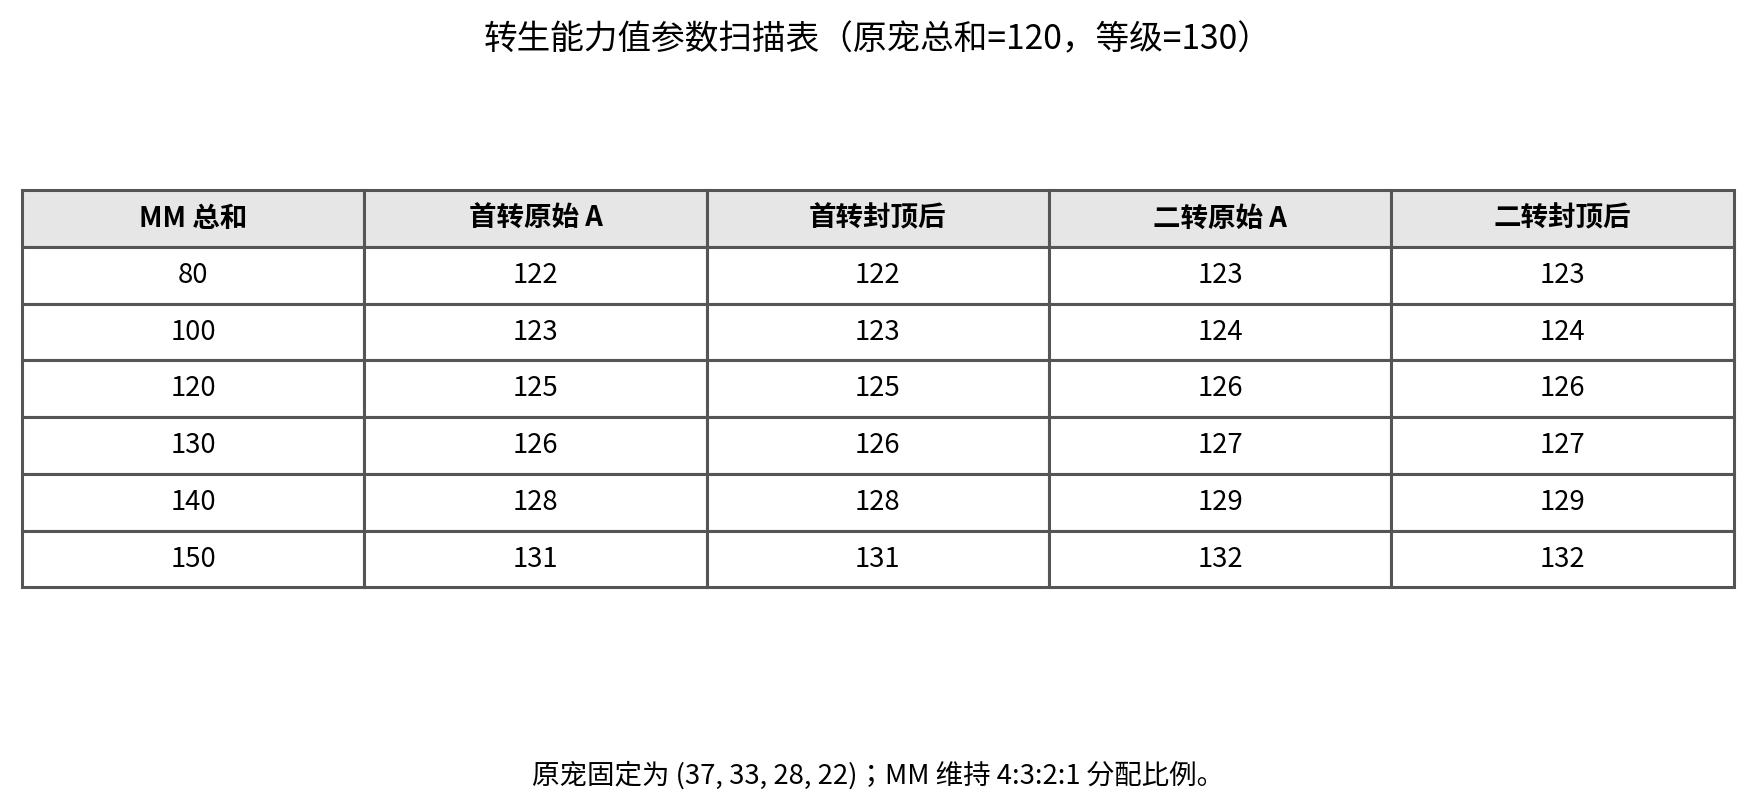
\includegraphics[width=0.82\textwidth]{figures/transmigration_scan_table.png}
    \caption{转生能力值参数扫描表。固定原宠成长总和为 $120$、宠物等级为 $130$，并令 MM 的四维分配保持 $4{:}3{:}2{:}1$ 比例。表中同时列出首转与二转的原始转生能力值和上限裁切结果，用于展示 Rank 表差异与能力上限的共同影响。}
    \label{fig:trans-scan-table}
\end{figure}

式~\eqref{eq:trans-new-alloc} 本身也是一个离散分配器，因为四维结果都分别向下取整，所以分配后的四项总和一般小于 $A^{*}$。这种“能力值存在，但落不到任何一维”的现象，正是转生页面中经常出现 1 至 3 点落差的根源。图~\ref{fig:trans-alloc-loss-table} 给出一个固定原宠与 MM 配置下的实证扫描，可以看到即使 $A^{*}$ 继续上升，四维总和也会以台阶方式增长，而不是逐点连续增长。

\begin{figure}[H]
    \centering
    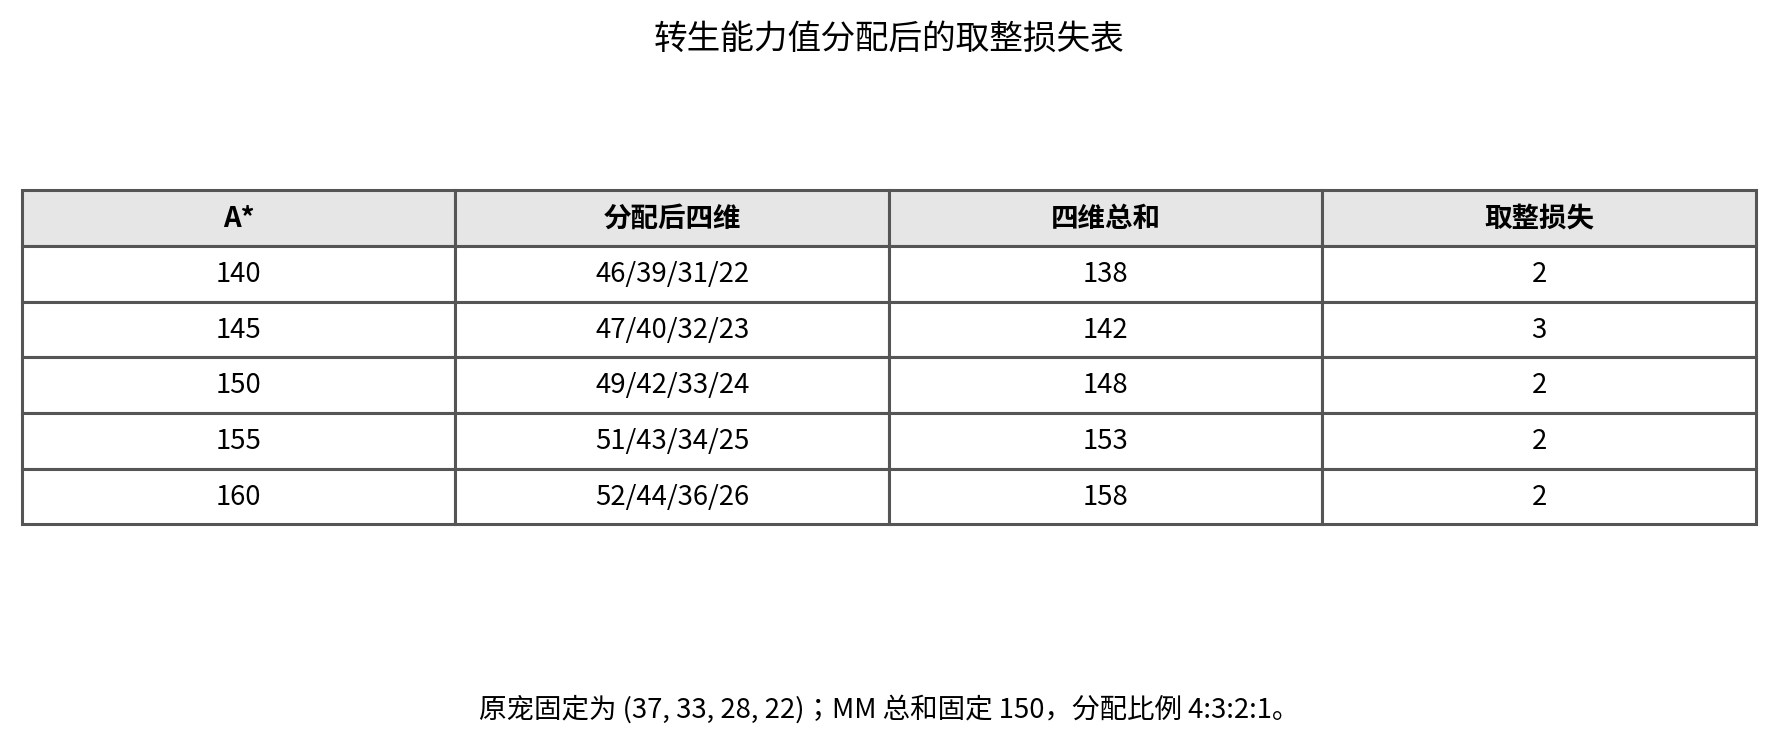
\includegraphics[width=0.82\textwidth]{figures/transmigration_alloc_loss_table.png}
    \caption{转生能力值分配后的取整损失表。固定原宠成长为 $(37,33,28,22)$、MM 总和为 $150$ 且分配比例为 $4{:}3{:}2{:}1$，展示不同 $A^{*}$ 在按权重分配并逐项向下取整后，四项总和与原能力值之间的差额。}
    \label{fig:trans-alloc-loss-table}
\end{figure}

\subsection{按权重分配到四项成长}

得到 $A^{*}$ 之后，系统并不会把它平均分到四维，而是按“原宠四倍权重、MM 一倍权重”的方式重新分配。记总权重为
\begin{equation}
    W = T_1 + 4T_2,
\end{equation}
则每一维的新成长率为
\begin{equation}
    g_i^{(new)} = \left\lfloor \frac{A^{*}(m_i + 4g_i)}{W} \right\rfloor, \qquad i=1,2,3,4.
    \label{eq:trans-new-alloc}
\end{equation}
式~\eqref{eq:trans-new-alloc} 解释了为什么 MM 更像“修方向”而不是“推翻原宠结构”：在同样的 $A^{*}$ 下，原宠原本偏向哪一维，新的成长档仍会显著保持这种偏向。

最后还必须强调，$\bm{g}^{(new)}$ 只是转生后的\emph{确定性基础成长率}，而不是最终宠物。它仍会经历上一章中的 $\pm2$ 波动、Rank 判定、出生随机加点和升级随机。因此，转生后的高等级属性依旧是一组分布，而不是单点。

\section{融合模型}

\subsection{主宠、副宠与低等级折扣}

融合模块的输入包括主宠与一只或两只副宠的等级及成长率。若某只参与融合的宠物等级低于 $80$，则其四维成长在进入后续步骤之前，需要先逐项做低等级折扣：
\begin{equation}
    g_i' = \left\lfloor 0.8 g_i \right\rfloor.
    \label{eq:fusion-level-discount}
\end{equation}
这里的关键不是 $0.8$ 这个系数本身，而是它\emph{先于后续贡献系数发生}。也就是说，主宠并不是“先乘 $0.6$ 再统一乘 $0.8$”，副宠也不是“先平均后再看是否低于 $80$ 级”，而是每只低等级宠物先单独完成一次截断，再进入主宠贡献或副宠平均的后续步骤。

\subsection{主宠贡献与副宠贡献}

设主宠折扣后的成长向量为 $\bm{g}^{(M)}$，副宠折扣后的成长向量分别为 $\bm{g}^{(S1)}$、$\bm{g}^{(S2)}$。若副宠数量为 $n_s\in\{1,2\}$，则先求逐项和
\begin{equation}
    s_i = \sum_{k=1}^{n_s} g_i^{(Sk)},
\end{equation}
再逐项做整数平均
\begin{equation}
    \bar{s}_i = \left\lfloor \frac{s_i}{n_s} \right\rfloor.
    \label{eq:sub-avg}
\end{equation}
随后，主宠贡献与副宠贡献分别为
\begin{equation}
    c_i^{(M)} = \left\lfloor 0.6 g_i^{(M)} \right\rfloor,
\end{equation}
\begin{equation}
    c_i^{(S)} = \left\lfloor 0.4 \bar{s}_i \right\rfloor.
    \label{eq:sub-contrib}
\end{equation}
最终蛋基础成长为
\begin{equation}
    b_i = c_i^{(M)} + c_i^{(S)}.
    \label{eq:egg-base}
\end{equation}
式~\eqref{eq:sub-avg} 与式~\eqref{eq:sub-contrib} 的顺序非常重要，因为“先平均再乘 $0.4$”与“先乘 $0.4$ 再平均”在整数系统中并不等价。当前实现与 \code{gmsv} 一致，明确采用前者。因此，融合模型本质上是一个逐步取整的离散算子，而不是一个可任意交换次序的线性组合。

\begin{figure}[H]
    \centering
    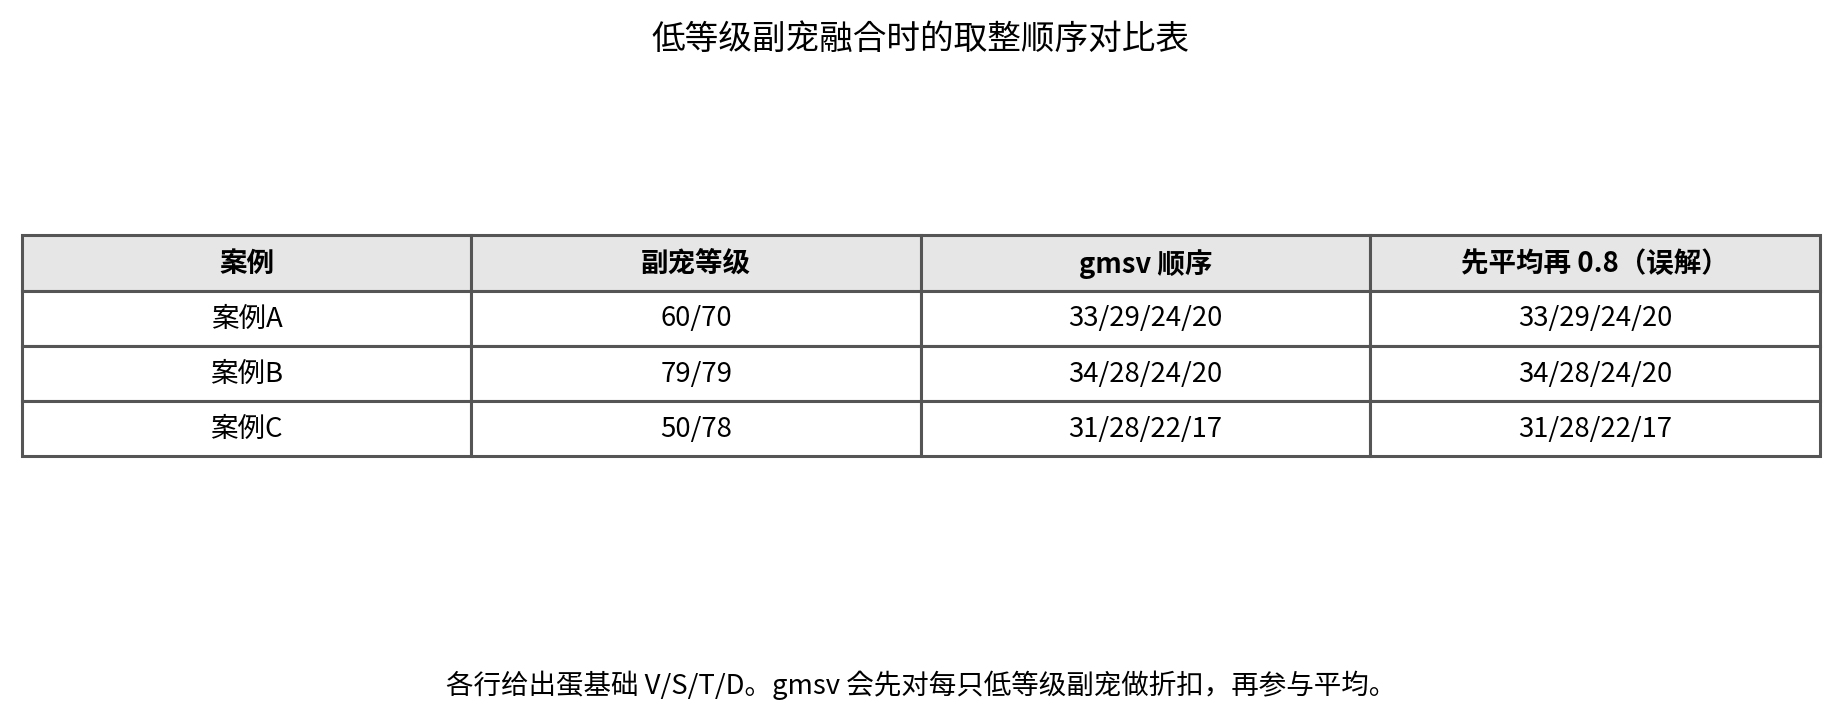
\includegraphics[width=0.86\textwidth]{figures/fusion_rounding_table.png}
    \caption{低等级副宠参与融合时的取整顺序对比。表中给出三组副宠案例，并比较 \code{gmsv} 实际采用的“各自先做 $0.8$ 折扣，再平均”与常见误解“先平均，再统一做 $0.8$ 折扣”所得到的蛋基础成长。可以看到，仅仅交换取整顺序就足以改变最终蛋面。}
    \label{fig:fusion-rounding-table}
\end{figure}

\section{蛋喂养模型}

\subsection{药效累加与折算}

蛋喂药的输入包括蛋基础成长 $\bm{b}$ 与一个 $4\times 5$ 的喂药方案矩阵。记第 $i$ 维在第 $\ell$ 级药上喂食的颗数为 $c_{i\ell}$，第 $\ell$ 级药的原始值为 $e_{\ell}$，则每一维的药效原始和为
\begin{equation}
    r_i = \sum_{\ell=1}^{5} c_{i\ell} e_{\ell}.
\end{equation}
在当前默认口径下，$e_{\ell}$ 依次为 $25,50,75,100,125$，且总喂食颗数固定为 $40$。原始药效不会直接加到成长档上，而是先折算为
\begin{equation}
    u_i = \min\left\{\left\lfloor \frac{7r_i}{1000} \right\rfloor,\,60\right\}.
    \label{eq:feed-fold}
\end{equation}
这一步对应“折算单项上限 $60$”。它说明高等级药和低等级药的效果虽然在线性原始值层面可相加，但一旦进入折算与上限，就会产生显著的离散差异。

\subsection{50 压缩与再分配}

记折算后的总和为
\begin{equation}
    U = \sum_{i=1}^{4} u_i.
\end{equation}
若 $U \le 50$，则直接令 $w_i=u_i$；若 $U>50$，则先做整体压缩：
\begin{equation}
    w_i = \left\lfloor \frac{50u_i}{U} \right\rfloor.
    \label{eq:work-cap}
\end{equation}
接下来，并不是把 $w_i$ 直接加到蛋基础成长上，而是再通过一轮“半折算 + 按比例回分配”生成孵化后成长。记
\begin{equation}
    T_1 = \sum_{i=1}^{4} w_i, \qquad T_2 = \sum_{i=1}^{4} b_i,
\end{equation}
并定义
\begin{equation}
    T = \left\lfloor \frac{T_1}{2} \right\rfloor + T_2.
\end{equation}
当前实现对每一维使用
\begin{equation}
    f_i = b_i + \left\lfloor \frac{w_i}{2} \right\rfloor,
\end{equation}
再计算增量
\begin{equation}
    \Delta_i = \left\lfloor \frac{f_i}{T} T_1 \right\rfloor,
\end{equation}
从而得到初步孵化成长
\begin{equation}
    h_i' = \operatorname{clip}_{[1,60]}\bigl(b_i + \Delta_i\bigr).
    \label{eq:hatch-pre}
\end{equation}
式~\eqref{eq:hatch-pre} 中最容易被忽略的细节是：系统使用的是 $w_i//2$ 和 $T_1//2$，而不是实数意义上的除以 $2$。因此，药效并入蛋成长时存在一层额外的整数损失，这也是喂药优化必须采用搜索而不是简单比例推算的原因之一。

\subsection{150 压缩与最终孵化成长}

记初步孵化成长总和为
\begin{equation}
    H' = \sum_{i=1}^{4} h_i'.
\end{equation}
若 $H' \le 150$，则最终孵化后成长直接取 $h_i=h_i'$；若 $H'>150$，则再施加一次总和压缩：
\begin{equation}
    h_i = \operatorname{clip}_{[1,60]}\left(\left\lfloor \frac{150h_i'}{H'} \right\rfloor\right).
    \label{eq:hatch-final}
\end{equation}
于是，当前工具中的“孵化后成长”本质上是由式~\eqref{eq:feed-fold}、式~\eqref{eq:work-cap}、式~\eqref{eq:hatch-pre} 和式~\eqref{eq:hatch-final} 共同决定的离散映射。它既不是药效与蛋成长的简单求和，也不是一个只需看总和的线性规划问题，而是同时受到单项上限、总和上限、比例回分配和多次向下取整约束的组合优化问题。

在默认参数 `40` 颗药、五级药原始值上限 `125` 的设定下，还有一个容易被忽略的事实：所有药的原始总和最多只有 $40 \times 125 = 5000$，因此折算后四维工作值总和满足
\begin{equation}
    \sum_i u_i \le \left\lfloor \frac{7 \times 5000}{1000} \right\rfloor = 35,
\end{equation}
从而式~\eqref{eq:work-cap} 中的 `50` 压缩在默认规则下实际上是休眠的。也就是说，当前默认喂药问题真正会起作用的总和约束，主要是后面的 `150` 孵化总和压缩，而不是前面的 `50` 工作值压缩。

\begin{figure}[H]
    \centering
    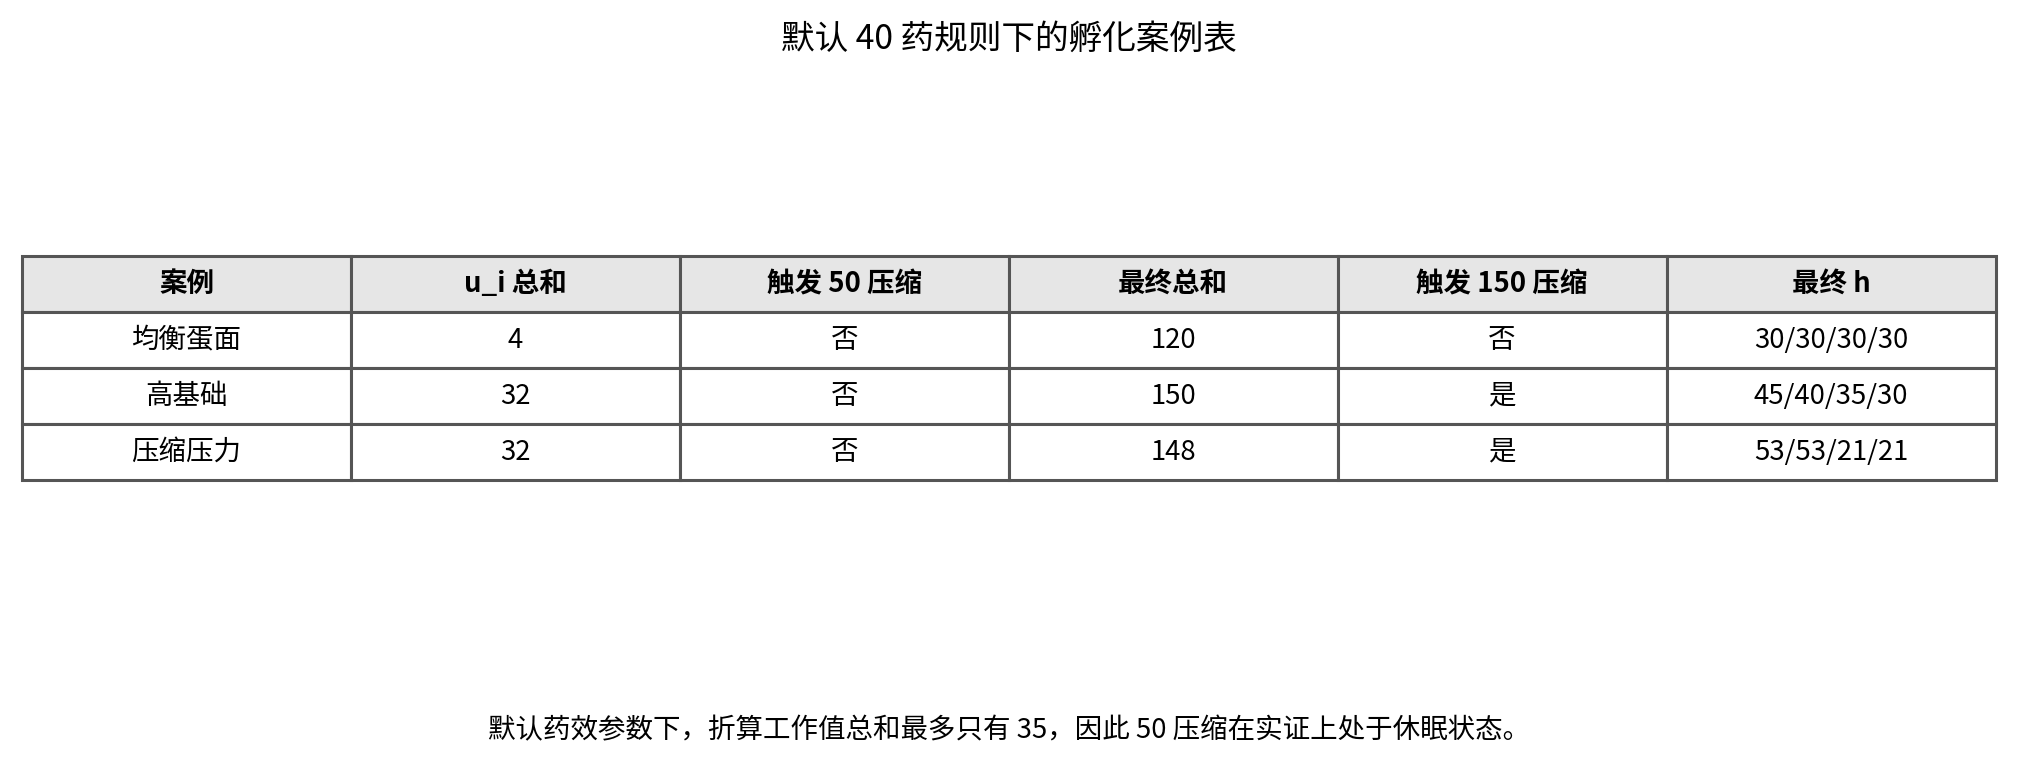
\includegraphics[width=0.9\textwidth]{figures/hatch_case_table.png}
    \caption{默认 `40` 药规则下的孵化案例表。表中列出不同蛋基础成长和喂药方案下的折算工作值总和、`50` 压缩是否触发、最终孵化总和以及 `150` 压缩是否触发。它直接展示了一个实证事实：在默认药效参数下，`50` 压缩不触发，而真正决定结果的常是最终 `150` 总和压缩。}
    \label{fig:hatch-case-table}
\end{figure}

若进一步把问题聚焦到“单项最终能否到 $60$”，则还会出现另一层阈值现象：即使某一维的喂药全部集中，只要其余三项总和过高，最终 `150` 压缩仍会把该维重新压回去。图~\ref{fig:hatch-threshold-table} 给出一个固定实验口径：把 `40` 颗五级药全部喂给敏捷维，并让其余三项基础成长尽量均分。表中列出的最小基础值阈值，正可以用来说明“为什么蛋面不到某个点，孵化后单项就上不去 $60$”。

\begin{figure}[H]
    \centering
    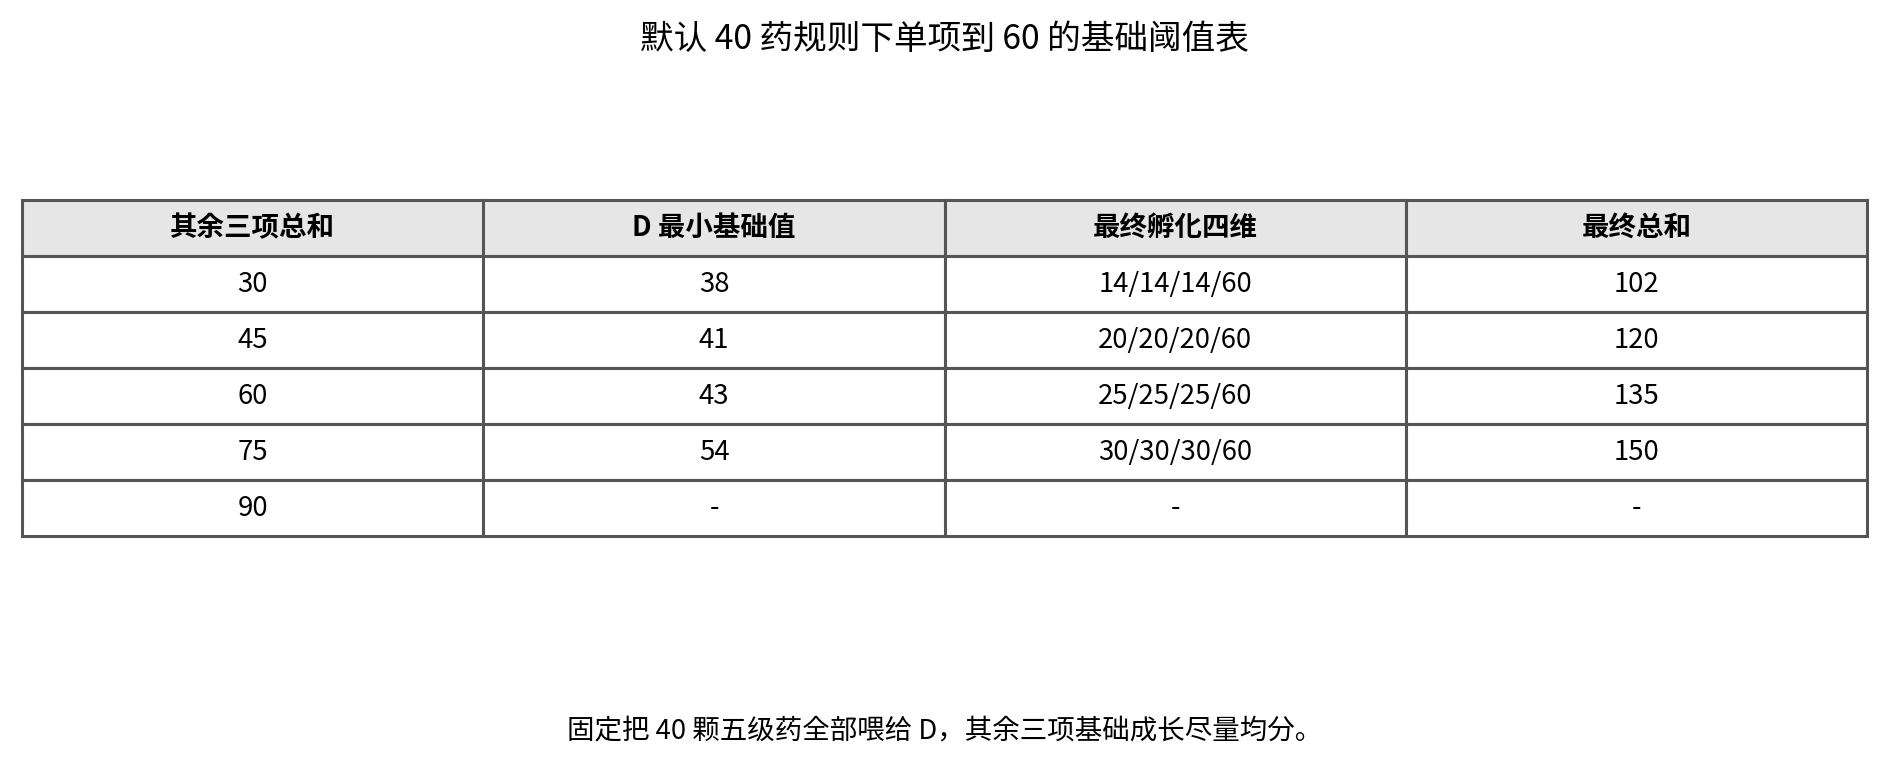
\includegraphics[width=0.84\textwidth]{figures/hatch_threshold_table.png}
    \caption{默认 `40` 药规则下单项到达 $60$ 的基础阈值表。固定把 `40` 颗五级药全部投入敏捷维，并令其余三项基础成长尽量均分，比较在不同“其余三项总和”下，敏捷维最终到达 $60$ 所需的最小蛋面基础值。}
    \label{fig:hatch-threshold-table}
\end{figure}

\section{孵化模型}

为了避免概念混乱，本文把“孵化”分成两个层次。第一层是当前工具所分析的\emph{确定性孵化成长}，也就是上一节得到的 $\bm{h}$；第二层是真正进入出生流程后的\emph{随机出生状态}，它还会叠加额外的随机扰动。对实际游戏过程而言，后者至少还可能包含四维独立的 $\pm2$ 波动、基于波动后总和的 Rank 判定，以及出生时的 $10$ 点随机加点。对当前论文和工具而言，主要优化对象是第一层，也就是不含出生后随机加点的孵化后成长。

这种分层处理有两个好处。第一，它把“喂药方案比较”与“出生运气比较”分开了：前者属于可控优化，后者属于随机结果。第二，它使得融合、喂药和普通成长之间的接口更加清晰。无论蛋来自哪种融合方案、喂了哪种药，最终都会先落到一个确定性的孵化成长向量 $\bm{h}$ 上，再由普通成长随机机制继续展开。

\section{养成链条的统一表示}

综合前述各节，本文将宠物养成系统写成如下统一流水线：
\begin{equation}
    \begin{aligned}
    \text{原宠} &\xrightarrow[]{\text{转生或保留}} \text{成长档} \xrightarrow[]{\text{融合}} \text{蛋基础成长 } \bm{b} \\
    &\xrightarrow[]{\text{喂药与孵化}} \text{孵化后成长 } \bm{h} \xrightarrow[]{\text{出生与升级随机}} \text{高等级面板}.
    \end{aligned}
\end{equation}
这条链的意义在于，它把原本散落在不同页面和不同源码函数中的机制统一成了一个状态变换序列。对工具开发而言，这意味着不同页面其实是在同一条链上截取不同节点；对后续战斗分析而言，这意味着命中、会心、先手和伤害所真正依赖的，不是某个孤立的喂药数值，而是整条养成流水线在终点处生成的有效成长与面板分布。

从研究角度看，本章最重要的结论不是某一条公式本身，而是所有这些公式共有的结构特征：它们几乎都不是连续线性过程，而是“先截断、再裁切、再按比例分配”的离散系统。也正因为如此，宠物培养问题天然适合被建模为离散优化与状态转移问题，而不是简单的线性加权问题。后文在讨论战斗表现与喂药最优方案时，将反复使用本章建立的这套离散流水线视角。
